% **************************** %
%          Slides GK           %
% **************************** %

\documentclass[10pt,fleqn]{beamer}
 
% **************************** %
%            Package           %
% **************************** %

% \usepackage{GarmirKhatch}
\usepackage{etex} % pour éviter erreurs de compilation avec tikz
\reserveinserts{20}

\usepackage[utf8]{inputenc}
\usepackage[T1]{fontenc}
\usepackage[french,english]{babel}
\usepackage[french]{layout}
\usepackage{lmodern}
\usepackage{ragged2e}
\usepackage{fancyhdr}
\usepackage{verbatim}
\usepackage{graphicx}
\usepackage{wrapfig}
\usepackage{url}
\usepackage{hyperref}
\usepackage{amsmath}
\usepackage{multirow}
\usepackage{multicol}
\usepackage{array}
\usepackage{colortbl}
\usepackage{comment}
\usepackage{tikz}
\usepackage{tikz-uml}
\usetikzlibrary{positioning, shadows}
\newcommand{\mo}{\textsc{Garmir~Khatch}}

% **************************** %
%          Préambule           %
% **************************** %
% Option pdf
\hypersetup{
      %pdfpagemode = FullScreen,
      pdfauthor   = {AMU FSI 2014},
      pdftitle    = {Présentation du projet TMS pour \mo},
      pdfsubject  = {Système de gestion des transports},
      pdfkeywords = {AMO, GK, TMS, CdC, DAT, PTI}
}
% Thème du pdf 
\usetheme{Warsaw}
% Logo de l'université d'Aix-Marseille
%\logo{\includegraphics[height=6mm]{logo}}
% Affiche les notes
%\setbeameroption{show notes}
% Blocks arrondies et ombrés
\setbeamertemplate{blocks}[rounded][shadow=true] 
% Balle pour la liste d'items
\setbeamertemplate{itemize item}[ball]
% Triangle pour la liste de sous items
\setbeamertemplate{itemize subitem}[triangle]
% Affiche l'ensemble du frame en gris clair
\beamertemplatetransparentcovered
% Faire apparaître un sommaire avant chaque section
\AtBeginSection[]{
	\begin{frame}
		\frametitle{Sommaire}
		\tableofcontents[currentsection, hideallsubsections]
	\end{frame}
}

% **************************** %
%        Page de garde         %
% **************************** %
\title[]{{\Large \textsc{\mo \\ Système de gestion des transports}}}
\author[\textsc{\mo - Système de gestion des transports}]{M2 FSIL - FSI}
\institute{Encadrant : M. Roland \textsc{Agopian}\\
Faculté des Sciences d'Aix-Marseille Université\\
Campus de Luminy}
\date{\scriptsize{ 27 mars 2014}}

% **************************** %
%       Corps du document      %
% **************************** %
\begin{document}
 
% **************************** %
%            Entête            %
% **************************** %
\begin{frame}
\begin{figure}
\centering

\includegraphics[scale=0.52]{Images/EnTeteSciences}
\end{figure}
\titlepage
\end{frame}

\begin{frame}
\frametitle{Sommaire}
\tableofcontents[hideallsubsections]
\end{frame}

\section*{Gantt général}

% Présentation sommaire : AMO -> ME + GANTT de ces 2 taches

\section[Mission d'AMO]{Mission d'AMO}
%Les termes AMO, MO, ME seront utilisés. Est-il nécessaire de les expliciter~?

\subsection{Mission d'AMO~: Jalonnements}
\begin{frame}
	\frametitle{Mission d'AMO~: Jalonnements}
\end{frame}

\begin{frame}
	\centering
	\begin{block}{Gestion de projet}
	\begin{enumerate}
		\item Étude de faisabilité\pause
		\item Expression du besoin\pause
		\item Validation du besoin\pause
		\item Réponse au besoin\pause
		\item Choix de la solution\pause
		\item Conception\pause
		\item Réalisation\pause
		\item Vérification\pause
		\item Livraison\pause
		\item Exploitation\pause
	\end{enumerate}
	\end{block}
\end{frame}
s

\subsection{Objectifs pour nous}

\begin{frame}
	\frametitle{Objectifs pour nous}
	\begin{block}{}
		Rédiger et fournir un cahier des charges de consultation au client
	\end{block}
\end{frame}

%Objectif~: Rédaction d'un cahier des charges de consultation


\subsection{Mission d'AMO~: Organisation}
\begin{frame}
	\frametitle{Mission d'AMO~: Organisation} \pause
	\begin{block}{L'organisation générale} \pause
	\begin{itemize}
	\item L'AMO : 2 groupes de 4 étudiants \pause
	\item La MO : Mr Agopian pour le compte d'une société fictive \mo \pause
	\item Réunion hebdomadaire avec le client
	\end{itemize}
	\end{block}
\end{frame}

% Présentation de l'Organisation générale~: 2 groupes de 4 étudiants en tant qu'AMO, la MO Agopian pour le compte d'une société fictive Gk.
%% Réunion chaque semaine. GANTT
%% Agopian mode client vs mode pédagogique.



\subsection{Mission d'AMO~: Présentation de \mo}
\subsubsection{Présentation de \mo}

\begin{frame}
	\frametitle {Présentation de \mo} 
	\begin{block}{Présentation générale} \pause
	\begin{itemize}
	\item L'une des plus grandes organisations humanitaires au monde \pause
	\item Agit avant, pendant et après les catastrophes et les urgences relatives à la santé \pause
	\item Puise sa force de son réseau de volontaires
	\end{itemize}
	\end{block}
\end{frame}

 %% Présentation de Gk et de son projet.
% Gestion de la planification, du suivi, documentaire.
\begin{frame}
\frametitle {Présentation de \mo} \pause
     \begin{figure}[htbp]
	\centering
	\begin{tikzpicture}
		% définition des styles
		\tikzstyle{metier}=[rectangle,draw,fill=yellow!50,text=black]
		\tikzstyle{support}=[rectangle,draw,fill=blue!50,text=black]
		\tikzstyle{supporte}=[->,>=latex,thick,rounded corners=4pt]
		% les nœuds
		\node[metier] (e) at (-3,-3) {Eau et sanitaire};
		\node[metier] (m) at (0,0.5) {Médecine};
		\node[metier] (d) at (3,-3) {Distribution};
		\node[support] (l) at (-2,-1.5) {Logistique};
		\node[support] (t) at (2,-1.5) {Télécoms};
		% les flèches
		\draw[supporte] (l) to[bend left] (t);
		\draw[supporte] (l) to[bend right] (e);
		\draw[supporte] (l) to[bend left] (m);
		\draw[supporte] (l) to[bend right] (d);
		\draw[supporte] (t) to[bend left] (l);
		\draw[supporte] (t) to[bend left] (e);
		\draw[supporte] (t) to[bend right] (m);
		\draw[supporte] (t) to[bend left] (d);
		% la légende
		\draw[supporte] (4,0) -- (7,0) node[midway,above]{Supporte};
	\end{tikzpicture}
	\caption{Dépendances entre les métiers}
\end{figure}  
\end{frame}

\subsubsection{Présentation du projet}

\begin{frame}
\frametitle {Présentation de \mo} \pause
\begin{block}{Processus de la logistique} \pause
\begin{enumerate}
\item Achat \pause
\item Stockage \pause
\item Transport
\end{enumerate}
\end{block}

\begin{block}{Fonctions clefs de la logistique} \pause
\begin{enumerate}
\item Planification/évaluation \pause
\item Acquisition/achat \pause
\item Gestion des entrepôts \pause
\item Organisations des transports \pause
\item Suivi et compte rendu
\end{enumerate}
\end{block}
\end{frame}

\subsubsection{Objectifs du projet}

\begin{frame}
\frametitle {Présentation de \mo} 
\begin{block}{Objectifs de la mission d'AMO pour \mo}
\begin{itemize}
\item Améliorer la qualité de ses services en se dotant d'une solution de type Transport Management System(TMS) 
\item Espérance de retour sur investissement
\end{itemize}
\end{block}
\end{frame}

 \begin{frame}
 \frametitle {Présentation de \mo} 
 
\begin{figure}[htbp] % Arbre à problèmes
	\centering
	\begin{tikzpicture} [
			node distance = 0.4cm, auto,font=\footnotesize,
			% STYLES
			every node/.style={node distance=1.7cm},
			% The comment style is used to describe the characteristics of each force
			comment/.style={rectangle, inner sep= 3pt, text width=2.8cm, node distance=0.2cm, font=\scriptsize\sffamily},
			% The force style is used to draw the forces' name
			force/.style={rectangle, draw, fill=black!10, inner sep=3pt, text width=2.8cm, text badly centered, minimum height=1cm, font=\bfseries\normalsize\sffamily}
		] 
		% Nodes
		\node [force] (confiance) {Confiance\\{\normalfont\footnotesize Envers \mo}};
		\node [force, above of=confiance] (transparent) {Transparence des informations\\{\normalfont\footnotesize Grâce au suivi détaillé}};
		%% Mj %% Bug avec 'X[cm] of transparent' -> Mise ne commentaire et réécriture sans
		\node [force, right=0.6cm of transparent] (serieux) {Sérieux\\{\normalfont\footnotesize Car on peut justifier à tout moment de l'utilisation des ressources}};
		\node [force, left=0.6cm of transparent] (pro) {Professionnalisme\\{\normalfont\footnotesize Notamment grâce à la planification et à l'utilisation optimale du matériel}};
		\node [force, below of=confiance, left=-0.2cm of confiance] (don) {Dons à l'organisation};
		\node [force, below of=confiance, right=-0.2cm of confiance] (benevolat) {Hausse du bénévolat};
%		\node [force, right] (serieux) {Sérieux\\{\normalfont\footnotesize Car on peut justifier à tout moment de l'utilisation des ressources}};
%		\node [force, left] (pro) {Professionnalisme\\{\normalfont\footnotesize Notamment grâce à la planification et à l'utilisation optimale du matériel}};
%		\node [force, below of=confiance, left] (don) {Dons à l'organisation};
%		\node [force, below of=confiance, right] (benevolat) {Hausse du bénévolat};
		% Draw the links between forces
		\path[->,thick]
			(don) edge (confiance)
			(benevolat) edge (confiance)
			(confiance) edge (transparent)
			(confiance) edge (serieux)
			(confiance) edge (pro);
		\end{tikzpicture} 
	\caption{Arbre à problème : Finalité du projet et retour sur investissement}
\end{figure}
 \end{frame}
 
 \begin{frame}
 \frametitle {Présentation de \mo}
 \begin{block}{Nature des prestations demandées}
 \mo recherche  un prestataire pour la réalisation d'une solution TMS, les prestations attendues ~:
 \begin{enumerate}
 \item la suite logicielle \pause
 \item le matériel \pause
 \item le service support
 \end{enumerate}
 \end{block} \pause
 \begin{block}{Parties concernées}
 \begin{enumerate}
 \item Directement: les logisticiens de \mo
 \item Indirectement: les victimes prises en charge
 \end{enumerate}
 \end{block}
 \end{frame}
 
 \begin{frame}
 \frametitle {}
 \end{frame}

\subsection{Déroulement de la mission}

\subsubsection{Déroulement de la mission}

\begin{frame}
\frametitle{Déroulement de la mission}
\begin{block}{Déroulement de la mission}
	\begin{enumerate}
	\item Recherche d'une norme
	\item Énoncé du besoin
	\item Expression fonctionnelle du besoin
	\item Cadre de réponse
	\end{enumerate}
	\end{block}
\end{frame}
  
\begin{frame}
	\frametitle{Énoncé du besoin}
	\begin{figure}[htbp]
	\centering
	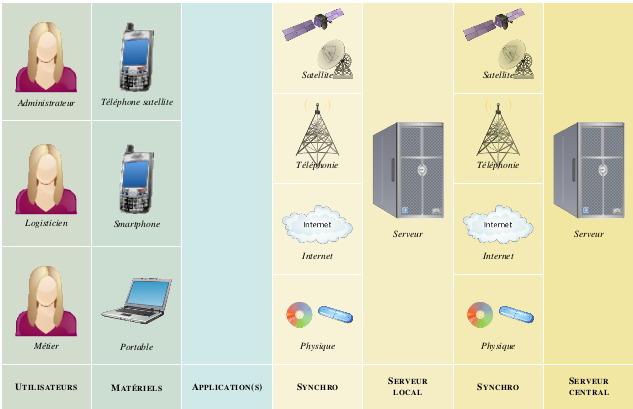
\includegraphics[scale=0.35]{Images/architecture.png}
	\caption{Architecture générale}
	\end{figure}
\end{frame}

\begin{frame}
\frametitle{Expression fonctionnelle du besoin}
\begin{block}{Fonctions de service et de contraintes}
\begin{itemize}
\item la localisation
\item l'interface utilisateur
\item les cas d'utilisations
\end{itemize}
\end{block}
\end{frame}

\begin{frame}
\frametitle{Les cas d'utilisations}
\end{frame}
% Jamais produit de cahier des charges. Nous étions initialement partit sur l'idée des spécifications.
%% Par manque d'expérience, des recherches nous ont menés à trouver une norme définissant le squelette d'un cahier des charges fonctionnel.
%% Norme et non loi. Première erreur a été de suivre sa lettre plutôt que son esprit.
%% PAQ pour le groupe 2.


\subsection{Conclusion}
\begin{frame}
	\frametitle{Conclusion}
\end{frame}

% A terme, les cdcf produit sont spécifiques à GK, à son métier et son contexte.
% Conclusion~: Comment cela s'est-il passé pour groupe1 \& 2~?



\section[Mission de ME]{Mission de ME}

\subsection{Mission de ME~: Jalonnements}
\begin{frame}
	\frametitle{Mission de ME~: Jalonnements}
\end{frame}

\begin{frame}
	\centering
	\begin{block}{Gestion de projet}
	\begin{enumerate}
		\item Étude de faisabilité\pause
		\item Expression du besoin\pause
		\item Validation du besoin\pause
		\item Réponse au besoin\pause
		\item Choix de la solution\pause
		\item Conception\pause
		\item Réalisation\pause
		\item Vérification\pause
		\item Livraison\pause
		\item Exploitation\pause
	\end{enumerate}
	\end{block}
\end{frame}
s

\include{Presentation_Me_Objectif_pour_nous}

\subsection{Organisation}
\begin{frame}
	\frametitle{Organisation}
	\begin{center}
	
\includegraphics[scale=1.2]{Images/organisation}
	\end{center}
\end{frame}


\subsection{Mission de ME~: Réponse technique à la disponibilité}
\begin{frame}
	\frametitle{Mission de ME~: Réponse technique à la disponibilité}
\end{frame}

% Fonctionnalité de disponibilité sans interruption~:
%% Client lourd, architecture générale.


\subsection{Mission de ME~: Réponse technique à la synchronisation}
\begin{frame}
	\frametitle{Mission de ME~: Réponse technique à la synchronisation}
\end{frame}


\subsection{Mission de ME~: Réponse technique à la sécurité}
\begin{frame}
	\frametitle{Mission de ME~: Réponse technique à la sécurité}
\end{frame}

% Fonctionnalité de sécurité~:
%% Problématique~: Authentification, gestion des droits utilisateurs et groupes utilisateurs.
%% Solutions possibles~: SGBDR, LDAP...
%% Solution choisie \& raisons~: LDAP
%%% Implémentation, problèmes rencontrés (librairie Windows, 32-64bits...), etc.


\subsection{Mission de ME~: Réponse technique au stockage des données}
\begin{frame}
	\frametitle{Mission de ME~: Réponse technique au stockage des données}
\end{frame}

% Fonctionnalité de données~:
%% Problématique~: Stockage des données.
%% Solutions possibles~: SGBDR, XML...
%% Solution choisie \& raisons~: SGBDR MySQL (rebondissement Postgres)
%%% Implémentation, problèmes rencontrés (Driver QMYSQL, solution de contournement SQLite...), etc.


\subsection{Mission de ME~: Réponse technique à la sauvegarde et reprise sur panne}
\begin{frame}
	\frametitle{Mission de ME~: Réponse technique à la sauvegarde et reprise sur panne}
\end{frame}

% Fonctionnalité de sauvegarde~:
%% Problématique~: Sauvegarde, reprise sur pannes...
%% Solutions possibles~:
%% Solution choisie \& raisons~:
%%% Implémentation, problèmes rencontrés (temps...), etc.


\subsection{Mission de ME~: Dossier d'Architecture Technique}
\begin{frame}
	\frametitle{Mission de ME~: Dossier d'Architecture Technique}
\end{frame}

% Conclusion~: tout ceci constitue la réponse technique aux besoins spécifiés dans le CdCF, de même que le DAT qui spécifie dans le détail l'architecture de ces solutions.



\subsection{Mission de ME~: Cahier de Recette}
\begin{frame}
	\frametitle{Mission de ME~: Cahier de Recette}
\end{frame}

% Cahier de recette (spécifié comme livrable par le CdCF).
%% Problématique~: Tester la solution, ses fonctionnalité, ses performances, son intégration, etc.



\subsection{Mission de ME~: Procédure d'Installation Technique}
\begin{frame}
	\frametitle{Mission de ME~: Procédure d'Installation Technique}
\end{frame}

% Procédure d'installation technique (spécifié comme livrable par le CdCF).



\subsection{Mission de ME~: Conclusion}
\begin{frame}
	\frametitle{Mission de ME~: Conclusion}
\end{frame}

% Listing des éléments de réponse demandés dans le CdCF, et cocher ceux rendus.



\end{document}
